\documentclass[12pt,a4paper]{article}
% math_setup.tex
% Essential Packages
\RequirePackage{etex}
\usepackage{comment}
\usepackage{etex}
\usepackage{listings}
\usepackage{amsmath}    % Advanced math typesetting
\usepackage{amsfonts}   % Math fonts
\usepackage{amssymb}    % Math symbols
\usepackage{amsthm}     % Theorem environment
\usepackage{mathtools}  % More symbols
\usepackage{tikz}       % For drawing diagrams
\usepackage{tikz-network}
\usepackage{pgfplots}
\usetikzlibrary{calc, arrows.meta, positioning, quotes}
\usepackage{mdframed}
\usepackage{float}
\usepackage{thmtools}
\usepackage{xcolor}
\usepackage{geometry}
\usepackage{fancyhdr}
\usepackage[colorlinks=true, linkcolor=blue, citecolor=green, urlcolor=red]{hyperref}
\usepackage{csquotes}
\usepackage[backend=biber, style=ieee]{biblatex}
\pgfplotsset{compat=1.18}
%\usepackage{mdframed}

% Wolfram Code Block
\lstdefinelanguage{Wolfram}{
    keywords={Sum, If, For, While, Do, Plot, Table, Range, Integrate, NIntegrate, D, Solve, NSolve, DSolve, NDSolve, LinearSolve, Expand, Factor, Simplify, FullSimplify, Module, Block, With},
    sensitive=true,
    morecomment=[l]{(*},
    morecomment=[s][\itshape]{(*}{*)},
    morestring=[b]",
    morestring=[b]',
}

\lstset{
    language=Wolfram,
    basicstyle=\ttfamily,
    keywordstyle=\color{blue}\bfseries,
    commentstyle=\color{green}\itshape,
    stringstyle=\color{red},
    showstringspaces=false,
    frame=single,
    breaklines=true,
    numbers=left,
    numberstyle=\tiny\color{gray},
    stepnumber=1,
    numbersep=5pt,
    backgroundcolor=\color{lightgray!20}
}

% add ref
\addbibresource{references.bib}
% Define colors
\definecolor{theoremcolor}{RGB}{230,230,250}  % Light purple
\definecolor{lemmacolor}{RGB}{240,248,255}    % Alice Blue
\definecolor{propcolor}{RGB}{240,255,240}     % Light green
\definecolor{corollarycolor}{RGB}{255,250,240} % Light orange
\definecolor{axiomcolor}{RGB}{255,240,245}    % Lavender blush
\definecolor{definitioncolor}{RGB}{240,255,255} % Light cyan
\definecolor{remarkcolor}{RGB}{245,245,245}   % Light gray
\definecolor{notationcolor}{RGB}{255,250,205}

% Boxed environments

\declaretheoremstyle[
    headfont=\normalfont\bfseries,
    bodyfont=\normalfont,
    headpunct={:},
    postheadspace=1em,
    mdframed={
        linecolor=black,
        backgroundcolor=definitioncolor,
        topline=true,
        bottomline=true,
        leftline=true,
        rightline=true,
        roundcorner=5pt
    }
]{boxeddefinitionstyle}

\declaretheorem[style=boxeddefinitionstyle, name=Definition]{definition}

\declaretheoremstyle[
    headfont=\normalfont\bfseries,
    bodyfont=\normalfont,
    headpunct={:},
    postheadspace=1em,
    mdframed={
        linecolor=black,
        backgroundcolor=theoremcolor,
        topline=true,
        bottomline=true,
        leftline=true,
        rightline=true,
        roundcorner=5pt
    }
]{boxedtheoremstyle}

% Theorem
\declaretheorem[style=boxedtheoremstyle, name=Theorem]{theorem}

% Lemma (adjust color)
\declaretheoremstyle[
    headfont=\normalfont\bfseries,
    bodyfont=\normalfont,
    headpunct={:},
    postheadspace=1em,
    mdframed={
        linecolor=black,
        backgroundcolor=lemmacolor,
        topline=true,
        bottomline=true,
        leftline=true,
        rightline=true,
        roundcorner=5pt
    }
]{boxedlemmastyle}
\declaretheorem[style=boxedlemmastyle, name=Lemma]{lemma}

% Proposition (adjust color)
\declaretheoremstyle[
    headfont=\normalfont\bfseries,
    bodyfont=\normalfont,
    headpunct={:},
    postheadspace=1em,
    mdframed={
        linecolor=black,
        backgroundcolor=propcolor,
        topline=true,
        bottomline=true,
        leftline=true,
        rightline=true,
        roundcorner=5pt
    }
]{boxedpropstyle}
\declaretheorem[style=boxedpropstyle, name=Proposition]{proposition}

% Corollary (adjust color)
\declaretheoremstyle[
    headfont=\normalfont\bfseries,
    bodyfont=\normalfont,
    headpunct={:},
    postheadspace=1em,
    mdframed={
        linecolor=black,
        backgroundcolor=corollarycolor,
        topline=true,
        bottomline=true,
        leftline=true,
        rightline=true,
        roundcorner=5pt
    }
]{boxedcorollarystyle}
\declaretheorem[style=boxedcorollarystyle, name=Corollary]{corollary}

% Axiom (boxed)
\declaretheoremstyle[
    headfont=\normalfont\bfseries,
    bodyfont=\normalfont,
    headpunct={:},
    postheadspace=1em,
    mdframed={
        linecolor=black,
        backgroundcolor=axiomcolor,
        topline=true,
        bottomline=true,
        leftline=true,
        rightline=true,
        roundcorner=5pt
    }
]{boxedaxiomstyle}
\declaretheorem[style=boxedaxiomstyle, name=Axiom]{axiom}

% Remark environment
\declaretheoremstyle[
    headfont=\normalfont\bfseries,
    bodyfont=\normalfont,
    headpunct={:},
    postheadspace=1em,
    mdframed={
        linecolor=black,
        backgroundcolor=remarkcolor,
        topline=true,
        bottomline=true,
        leftline=true,
        rightline=true,
        roundcorner=5pt
    }
]{remarkstyle}
\declaretheorem[style=remarkstyle, name=Remark, numbered=no]{remark}
% Normal, non-italic environments
\declaretheoremstyle[
    headfont=\normalfont\bfseries,
    bodyfont=\normalfont,
    headpunct={:},
    postheadspace=1em,
]{normalstyle}

% Notation environment
\declaretheoremstyle[
    headfont=\normalfont\bfseries,
    bodyfont=\normalfont,
    headpunct={:},
    postheadspace=1em,
    mdframed={
        linecolor=black,
        backgroundcolor=notationcolor,
        topline=true,
        bottomline=true,
        leftline=true,
        rightline=true,
        roundcorner=5pt
    }
]{boxednotationstyle}
\declaretheorem[style=boxednotationstyle, name=Notation]{notation}


% Note environment (more noticeable, with separators, no background, no end symbol)
\newenvironment{note}[1][]
    {\par\vspace{0.5em}\noindent\rule{\textwidth}{0.4pt}\par\vspace{0.5em}%
    \textbf{Note\if\relax\detokenize{#1}\relax\else: #1\fi}\par}
    {\par\vspace{0.5em}\noindent\rule{\textwidth}{0.4pt}\par\vspace{0.5em}}

\declaretheorem[style=normalstyle, name=Note, numbered=no]{oldnote}

\declaretheorem[style=normalstyle, name=Example]{example}
\declaretheorem[style=normalstyle, name=Exercise]{exercise}
\declaretheorem[style=normalstyle, name=Statement]{statement}
\declaretheorem[style=normalstyle, name=Solution, numbered=no]{solution}

% Proof environment (normal, non-italic, with QED symbol)
\declaretheoremstyle[
    headfont=\normalfont\bfseries,
    bodyfont=\normalfont,
    headpunct={:},
    postheadspace=1em,
    qed=$\blacksquare$
]{proofstyle}

\declaretheorem[style=proofstyle, name=Proof]{customproof}

% Shorthand
\newcommand{\vect}[1]{\mathbf{#1}} % For regular vectors
\newcommand{\uvec}[1]{\hat{\mathbf{#1}}} % For unit vectors
\newcommand{\prob}[1]{
    \section*{Problem #1}
}
\newcommand{\R}{\mathbb{R}} % Real numbers
\newcommand{\Z}{\mathbb{Z}} % Integers
\newcommand{\C}{\mathbb{C}} % Complex numbers
\newcommand{\N}{\mathbb{N}} % Natural numbers
\newcommand{\Q}{\mathbb{Q}} % Rational numbers
\newcommand{\Hq}{\mathbb{H}} % Quaternions
\newcommand{\F}{\mathbb{F}} % Finite fields
\newcommand{\Proj}{\mathbb{P}} % Projective space
\newcommand{\K}{\mathbb{K}} % Arbitrary field
\newcommand{\T}{\mathbb{T}} % Torus or sometimes denoted for Topological space
\newcommand{\A}{\mathbb{A}} % Affine space
\newcommand{\0}{\mathbf{0}} % Zero vector
\newcommand{\mbf}[1]{\mathbf{#1}} 
\newcommand{\mat}[1]{\mathbf{#1}}
\newcommand{\adj}{\operatorname{adj}}
\newcommand{\dom}[1]{
    \operatorname{dom}(#1)
}




% Layout
\geometry{a4paper, margin=1in}
\pagestyle{fancy}
\fancyhf{}
\rhead{\today}
\lhead{\textbf{ENG1005 Engineering Mathematics}}
\rfoot{Page \thepage}


\begin{document}
\title{ENG1005 Week1 Workshop Problem Set Solutions}
\author{Yang Xingyu (33533563)}
\date{\today}
\maketitle

\section*{Problem 1, 2}
\begin{solution}
We are provided that:
\begin{itemize}
    \item The incoming ray, reflected ray, and the normal vector of the solar panel are co-planar.
    \item The angle between reflected ray and the normal to the plane equals to the angle between incoming ray and the normal vector of the plane.
\end{itemize}
The first statement allows us to build up a Cartesian Coordinate of the model, since we can take it as a segmentation of the 3D model (a 2D model that simplifies the model). This is because, the normal vector is co-planar to the vertical segment (a line) of the mirror plane. Hence, all four elements ($\uvec{a}_i,\uvec{a}_r, \uvec{n}$ and the segment line of mirror plane) are all co-planar, and we can build up the coordinate with some point $o$ on the solar panel, where $\uvec{a}_i$ intersects $\uvec{a}_r$, as the origin, using normal base vectors: $\uvec{i} = (1,0)$and $\uvec{j} = (0,1)$.
The second statement is equivalent to say that the angles formed by the incoming and reflected ray are symmetrical with respect to the normal vector, and thus, we can draw the diagram below to show this system in $\mathbb{R}^2$, where $\angle \theta_i = \angle \theta_r$.
\begin{figure}[H]
    \centering
    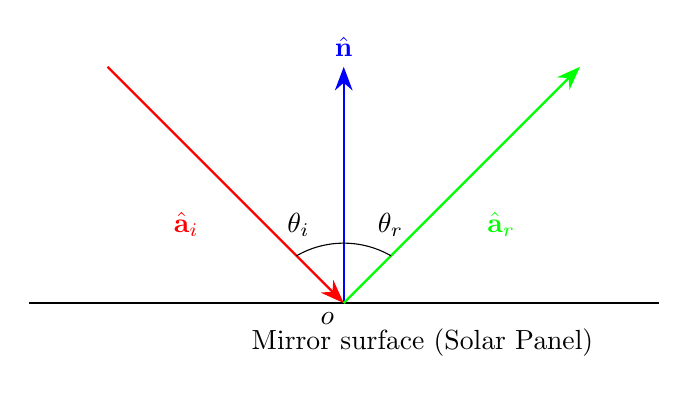
\begin{tikzpicture}[scale=2]
        % Mirror surface
        \draw[thick] (-2,0) -- (2,0);
         \node[anchor=north east] at (0,0) {$o$};
        % Normal vector
        \draw[-{Stealth[length=3mm]}, blue, thick] (0,0) -- (0,1.5) node[above] {$\uvec{n}$};
        
        % Incident ray
        \draw[-{Stealth[length=3mm]}, red, thick] (-1.5,1.5) -- (0,0) node at(-1,0.5) {$\uvec{a}_i$};
        
        % Reflected ray
        \draw[-{Stealth[length=3mm]}, green, thick] (0,0) -- (1.5,1.5) node at(1,0.5) {$\uvec{a}_r$};
        
        % Angle of incidence
        \draw (-0.3,0.3) arc (120:90:0.6) node[midway, above left] {$\theta_i$};
        
        % Angle of reflection
        \draw (0.3,0.3) arc (60:90:0.6) node[midway, above right] {$\theta_r$};
        
        % Label for mirror surface
        \node[below] at (0.5,-0.1) {Mirror surface (Solar Panel)};
    \end{tikzpicture}
    \caption{Visualization of Model}
\end{figure}
\begin{remark}
    Note that, rigorously, $\theta_i$ is the angle between $-\uvec{a}_i \text{ and } \uvec{n}$.
\end{remark}
\end{solution}


\section*{Problem 3}
Given the following corollary from the Fundamental Law of Reflection in Optics, we need to verify the two statements provided earlier.
\begin{corollary}[A Result from Fundamental Law of Reflection in Optics]
    If $\hat{\mathbf{a}}_i$ is a unit vector in the direction of an incoming light ray onto a plane mirror with normal $\hat{\mathbf{n}}$, then the mirror reflection law says that the direction of the reflected ray $\hat{\mathbf{a}}_r$ is given by
    \begin{equation}\label{given}
        \hat{\mathbf{a}}_r=\hat{\mathbf{a}}_i-2\left(\hat{\mathbf{a}}_i \cdot \hat{\mathbf{n}}\right) \hat{\mathbf{n}}.
    \end{equation}

\end{corollary}

Now we approach to prove the first statement that $\uvec{a}_i$, $\uvec{a}_r$, and $\uvec{n}$ are co-planar.
\begin{proof}
    By equation \ref{given}, we know that $\uvec{a}_r$ is a linear combination of $\uvec{n}$ and $\uvec{a}_i$. This implies that $\uvec{a}_r$ must be co-planar with $\uvec{n}$ and $\uvec{a}_i$.

    $\uvec{a}_r$ is a linear combination of $\uvec{a}_i$ and $\uvec{n}$ can be interpreted as, $$\exists \text{ some plane }\alpha \text{ defined by }\uvec{a}_i \text{ and }\uvec{n}, \text{ such that } \uvec{a}_r \in \alpha.$$

    We also have $\uvec{a}_i \in \alpha$ and $\uvec{n} \in \alpha$, therefore
    $$\begin{cases}
        \uvec{a}_r \in \alpha\\
        \uvec{a}_i \in \alpha\\
        \uvec{n} \in \alpha
    \end{cases}
    \implies
    \{\uvec{a}_r, \uvec{a}_i, \uvec{n}\} \subseteq \alpha.$$

    We have hence shown the existence of the plane that we call $\alpha$, where the three vectors are co-planar.
    \end{proof}
    \begin{remark}
        Actually we can also prove its uniqueness by an axiom of Euclidean space. 
        \begin{axiom}[Unique Plane Axiom]
        Through any three non-collinear points, there exists exactly one plane.
    \end{axiom}
    \begin{proof}
        Since $\uvec{a}_i$ and $\uvec{n}$ are not collinear and $\uvec{a}_r$ lies in the plane they define, we can always find two non-collinear points from $\uvec{a}_i$ and $\uvec{n}$ (one from each). Next, we find the third non-collinear point from $\uvec{a}_r$, so that the three points are pairwise non-collinear. Hence, the uniqueness is proven.
    \end{proof}
    
    \end{remark}
   
    
    By Unique Plane Axiom, we have confirmed that $\exists$ a unique plane $\alpha$, where  Hence, $\uvec{a}_i$, $\uvec{a}_r$, and $\uvec{n}$ are co-planar. The first statement is proven.
    
    
    Next, we will prove $\angle \theta_i=\angle \theta_r$ by the identity from equation \ref{given}.
    \begin{proof}
        To show that $\angle \theta_i=\angle \theta_r$, we may use the trigonometry identity that
        \begin{equation}\label{trigeq}
            \angle a=\angle b \iff \cos{a} = \cos{b}.
        \end{equation}
        \begin{remark}
            We have the above because circularity and negative angle are not considered here. This is because in the scenario of a ray hits the solar panel, we always have the relations 
            $$0 \leq \angle \theta_i \leq \frac{\pi}{2} \quad \text{and} \quad 0 \leq \angle \theta_r \leq \frac{\pi}{2}.$$
            This is due to the nature of this optical problem.
            
            Mathematically, the two angles are in the same cycle of $\cos$ function, as $T(\cos{x}) = 2 \pi$, ensuring that equation \ref{trigeq} holds.
        \end{remark}
        
    Here, we introduce a new lemma.
    \begin{lemma}
    Given two unit vectors $\uvec{a}\text{ and }\uvec{b}$, and the angle between the two vectors is $\theta$. Then
    $$\cos{\theta} = \frac{\uvec{a}\cdot \uvec{b}}{|\uvec{a}||\uvec{b}|} = \uvec{a}\cdot \uvec{b}.
    $$ 
    \end{lemma}
We consider the value of \(\cos \theta_r\):
\[
\cos \theta_r = \frac{\uvec{a}_r \cdot \uvec{n}}{|\uvec{a}_r||\uvec{n}|},
\]
By lemma 1, this simplifies to:
\[
\cos \theta_r = \uvec{a}_r \cdot \uvec{n}.
\]
Using the reflection formula \(\uvec{a}_r = \uvec{a}_i - 2 (\uvec{a}_i \cdot \uvec{n}) \uvec{n}\), we have:
\[
\cos \theta_r = [\uvec{a}_i - 2 (\uvec{a}_i \cdot \uvec{n}) \uvec{n}] \cdot \uvec{n}.
\]
Expanding the dot product and using distributive and associative properties, we get:
\[
\cos \theta_r = \uvec{a}_i \cdot \uvec{n} - 2 (\uvec{a}_i \cdot \uvec{n}) (\uvec{n} \cdot \uvec{n}).
\]
Since \(\uvec{n} \cdot \uvec{n} = |\uvec{n}|^2 = 1\), this simplifies to:
\[
\cos \theta_r = \uvec{a}_i \cdot \uvec{n} - 2 (\uvec{a}_i \cdot \uvec{n}) = -(\uvec{a}_i \cdot \uvec{n}).
\]

Because $-\uvec{a}_i$ and $\uvec{n}$ forms \(\theta_i\), and $-\uvec{a}_i$ is the vector with same magnitude but opposite direction of $\uvec{a}_i$, so \(\cos \theta_i = -\uvec{a}_i \cdot \uvec{n}\).

By lemma 1 again, we can thus show that:
\begin{equation}\label{obtain}
\cos \theta_r = -\cos \theta_i + 2\cos \theta_i = \cos \theta_i.
\end{equation}

By equation \ref{trigeq} and equation \ref{obtain}, we have:
\[
\angle \theta_i = \angle \theta_r.
\]
This completes the proof.
\end{proof}
We have shown that  $\text{equation \ref{given} }\text{implies the two statements given.}$

\section*{Problem 4}
\begin{solution}
    The normal vector $\uvec{n}$ of the mirror when it is in the resting position (initial position) is $(1,0,0)$.
    This can be deduced from what is mentioned in the material that 
    \begin{quote}
        \textit{In its initial resting position, the mirror has its normal pointing due East.}
    \end{quote}
     Because the $x$-axis points to the east, so we must have some unit vector $\uvec{n}=(n_x, n_y, n_z)$, where $|\uvec{n}| = \sqrt{{n_x}^2 + {n_y}^2 + {n_z}^2} = 1$, which holds if and only if $n_x = 1$.
\end{solution}

\section*{Problem 5}
    \begin{solution}
        By the normal vector we obtained from last question, we can confirm that the sunlight goes into the origin of the coordinate system. This is because the nature of the scenario that the incoming and reflected light intersects at where the normal vector of the plane stretches out. As $\uvec{n}$ is towards east and $|\uvec{n}| = 1$, we know that the intersection of $\uvec{a}_i$ and $\uvec{a}_r$ is $(0,0,0)$, i.e., the origin of the 3D coordinate system.

        It is mentioned that
        \begin{quote}
            \textit{The sun appears to be in the direction of the vector $(10, 2, 11)$.}
        \end{quote}
        This can be interpreted as that, the position vector of the sun $\vect{s}:= (10, 2, 11).$
        
        By the definition of position vector.
        \begin{definition}[Position vector]
        A \emph{position vector} of a point \( P \) in a Euclidean space is a vector that originates from the origin of the coordinate system and terminates at the point \( P \). Mathematically, if the coordinates of \( P \) are \( (x, y, z) \) in a three-dimensional space, then the position vector \( \mathbf{r} \) can be written as:
        \[
        \mathbf{r} = x \hat{\mathbf{i}} + y \hat{\mathbf{j}} + z \hat{\mathbf{k}}
        \]
        where \( \hat{\mathbf{i}}, \hat{\mathbf{j}}, \) and \( \hat{\mathbf{k}} \) are the unit vectors in the direction of the \( x \)-axis, \( y \)-axis, and \( z \)-axis, respectively.
        \end{definition}
        This lead us to the special case that the direction vector of incoming ray emitted by the sun is exactly $-\vect{s} = (-10, -2, -11)$, since we know the light goes into the origin $o = (0,0,0)$ from the sun.
        Thus, $\uvec{a}_i = \frac{-\vect{s}}{|-\vect{s}|} = -\frac{1}{15}\vect{s} = \left( -\frac{2}{3}, -\frac{2}{15}, -\frac{11}{15} \right)$.
    \end{solution}

    \section*{Problem 6}
    \begin{solution}
     Since we have obtained $\uvec{a}_i$ and $\uvec{n}$, we can use equation \ref{given} to get $\uvec{a}_r$.
     
        Given:
\[
\uvec{a}_i = \left( -\frac{2}{3}, -\frac{2}{15}, -\frac{11}{15} \right)
\]
and
\[
\uvec{n} = (1, 0, 0)
\]

First, we compute the dot product \(\uvec{a}_i \cdot \uvec{n}\):
\[
\uvec{a}_i \cdot \uvec{n} = \left( -\frac{2}{3} \right) \cdot 1 + \left( -\frac{2}{15} \right) \cdot 0 + \left( -\frac{11}{15} \right) \cdot 0 = -\frac{2}{3}
\]

Next, we substitute this into the reflection equation:
\[
\uvec{a}_r = \left( -\frac{2}{3}, -\frac{2}{15}, -\frac{11}{15} \right) - 2 \left( -\frac{2}{3} \right) (1, 0, 0)
\]

This simplifies to:
\[
\uvec{a}_r = \left( -\frac{2}{3} + \frac{4}{3}, -\frac{2}{15}, -\frac{11}{15} \right) = \left( \frac{2}{3}, -\frac{2}{15}, -\frac{11}{15} \right)
\]

Therefore, the direction vector of the reflected ray is:
\[
\uvec{a}_r = \left( \frac{2}{3}, -\frac{2}{15}, -\frac{11}{15} \right)
\]
    \end{solution}

\section*{Problem 7}
\begin{solution}
We can define the parametric equation of the reflected ray's trace, since we know it passes $(0,0,0)$ and we have one of its direction vector $\uvec{a}_r$.
So we have 
$$
l_{r} := ( 0,0,0) +t\hat{a}_{r} = \left( \frac{2}{3}t, -\frac{2}{15}t, -\frac{11}{15}t \right)
$$

The ray hit the collector if and only if $(-100,100,50)$ is on that line. We can verify whether this holds by substituting the coordinates of the point into the parametric equation and solving for \( t \).
We have,
$$
\begin{cases}
\frac{2}{3}t = -100 \\
-\frac{2}{15}t = 100 \\
-\frac{11}{15}t = 50
\end{cases}
$$
which has no solution.

Thus, the reflected light will not hit the collector.
\end{solution}

\section*{Problem 8}
\begin{solution}
When the reflected light hit on the collector, the unit vector of the reflected ray, $\uvec{a}_r$ satisfies
$$\uvec{a}_r =\frac{1}{150}(-100,100,50) = \left(-\frac{2}{3}, \frac{2}{3}, \frac{1}{3} \right).$$

Another important implied information is that, while the plane rotates, point of incidence and the sun remains still, only the normal vector $\uvec{n}$ changes, so we still have the same incoming ray vector $\uvec{a}_i = \left( -\frac{2}{3}, -\frac{2}{15}, -\frac{11}{15} \right)$.
\begin{remark}
We can actually strictly prove that we still have the same $\uvec{a}_i$ after the rotation.

The rotation of the solar panel in this model is obviously a rigid transformation, as the property of the solar panel itself, e.g., its size, does not change after the transformation. To provide more mathematical background, we introduce the definition.
\begin{definition}[Rigid Transformation]
A \emph{rigid transformation} (also known as \textit{Euclidean transformation}) is a geometric transformation that preserves the distance between any two points, thereby preserving the shape and size of geometric figures. It can be represented as a combination of a rotation and a translation.

Mathematically, a rigid transformation is a mapping \( T: \R^n \to \R^n \), which can be defined as:
$$
\mathbf{y} = T(\mathbf{x}) = \mathbf{R}\mathbf{x} + \mathbf{t},
$$
where
\(\mathbf{x}\) is the position vector of a point before transformation,
\(\mathbf{y}\) is the position vector of the point after transformation,
\(\mathbf{R}\) is a rotation matrix,
\(\mathbf{t}\) is a translation vector.

\end{definition}

Now we'll manage to show that given that the source of light does not change, rotating the panel will not change unit vector of the incident light.
\begin{proof}
    As per our assumption in this model, the incident light, reflected light, and the normal vector meets each other at the origin $o=(0,0,0)$. We also know that, the direction vector of the incoming light to the plane is $o - \vect{s} = -\vect{s}$, where $\vect{s}$ is the position vector of the sun. Hence, 
    $$\uvec{a}_i = \frac{-\vect{s}}{|-\vect{s}|} \text{ is static in the transformation}\iff -\vect{s} \text{ is constant.}$$

    It is already known that $\vect{s}$ is stagnant in the coordinate system during the rotation, so to prove the statement, we only need to show that the origin $o$ is constant before and after the transformation. This can be proven in many ways.

    We first attempt to prove it by the nature of the rotation. We have confirmed that the rotation of the solar panel can be categorized as a rigid transformation in $\R^3$, and there is no any translation of the plane in the space, i.e., the translation vector $\vect{t}$ here in this scenario, is a zero vector. 
    
    Therefore, the result of rotating the origin $o$ is a zero vector multiplied by some rotation matrix $\vect{R}$, which yields a new zero vector. This can be practically interpreted as: the origin keeps in its initial position, and is thus, not affected by the transformation (rotation).
    \end{proof}
    We can also show this more neat and clean by \textbf{contradiction}. 
    
   \begin{proof}
    Suppose that $o$ will be transformed by the rotation, then the coordinates of all other points on the plane will be changed, as their coordinates are defined by their relative position to the origin of the 3D system, leading us to a completely new coordinate system, which contradicts the fact that this model is built in a consistent coordinate system. Thus, $o$ must not be transformed by the rotation.
   \end{proof}
   
I also came out an interesting constructive proof.

\begin{proof}
    As per the definition of rigid transformation:
    \begin{quote}
        \textit{A rigid transformation is a geometric transformation that preserves the distance between any two points.}
    \end{quote}
    The distance between any two points on the plane will not change before and after the rotation. Now, consider a random point ${p}=(p_x,p_y,p_z)$ on the plane before the transformation, and the corresponding point ${p'} = (p'_x,p'_y,p'_z)$ after the transformation.

    Since the transformation is rigid, the distance from the origin $o$ to ${p}$ must equal the distance from the new origin $o’$ to ${p'}$ (position of $o'$ is measured by the relative position to the previous $o = (0,0,0)$ in the same system,) but we do not know whether $o' = (0,0,0)$. Mathematically, that is:
    \[
    |{p} - o| = |{p'} - o'|.
    \]
    By the property zero vector.
    \[
    |p| = |p'- o'|
    \]
    Note that, we must have $|p| = |p'|$, because rotation does not change the distance of a point to the origin. Just like you can rotate the same vector in $\R^2$ in any desired direction without changing its length, which can be easily introduced to $\R^3$.

    Now we have
    $$
    \begin{cases}
        |p| = |p'- o'|\\ 
        |p| = |p'|
    \end{cases}
    \implies 
    |p'| = |p'- o'|
    $$
    So, $p' - o' = p'$ or $p' - o' = -p'$.

    The first case directly implies that $o' = (0,0,0)$, and thus shows that the object is stagnant at $(0,0,0)$ when rotated.

    Now we consider the second case.
     \[
    {p'} - {o'} = -{p'} \implies {o'} = 2{p'}.
    \]
    If this case holds, it implies that each point \( \mathbf{p'} \) would have to be its own mirror image about \( \mathbf{o'} \), effectively meaning that all points would be flipped across \( \mathbf{o'} \). This contradicts the fact that we only rotate, but not translate the plane. 
    \begin{note}
        Physically and practically, it also doesn't make any sense, since this is flipping the panel completely, that is, rotating 180 degrees, while usually only one side of the panel is designed for receiving the light.
    \end{note}
    We thus can refute this case.

    Therefore, $o' = (0,0,0)$ must holds, i.e., the origin does not move under the rigid transformation involving only rotation.
\end{proof}
   Hence, we have confirmed the consistency of $\uvec{a}_i$ in the model by showing the point of incidence is constant in the rotation.


We can generalize this to a more useful result in Euclidean space.
\begin{corollary}(Invariance of Origin in Rotation)
    In any Euclidean space $\R^n$, any rigid transformation that involves only rotation (i.e., $\vect{t} = \0$.) will never change the coordinates of the origin, so as the point on the origin, in a consistent coordinate system.
\end{corollary}
\end{remark}

Now, to find $\uvec{n}$, all we need to do is to rearrange equation \ref{given}
to a way that is easy to calculate $\uvec{n}$.
\begin{equation}
\uvec{n} = \frac{\uvec{a}_i - \uvec{a}_r}{2 (\uvec{a}_i \cdot \uvec{n})}
\end{equation}
Among which, $\uvec{a}_r = \left(-\frac{2}{3}, \frac{2}{3}, \frac{1}{3} \right)$, $\uvec{a}_i = \left( -\frac{2}{3}, -\frac{2}{15}, -\frac{11}{15} \right)$, and we suppose $\uvec{n} = (n_x, n_y, n_z)$.
\begin{equation}
\uvec{n} = \frac{\left( 0, -\frac{4}{5}, -\frac{16}{15} \right)}{2 \left( \left( -\frac{2}{3} \right) n_x + \left( -\frac{2}{15} \right) n_y + \left( -\frac{11}{15} \right) n_z \right)}
\end{equation}
Expand and write it in column vector form we have:

\begin{equation}
\left( \left( -\frac{4}{3} \right) n_x + \left( -\frac{4}{15} \right) n_y + \left( -\frac{22}{15} \right) n_z \right)
\left[ \begin{array}{c}
n_x \\
n_y \\
n_z
\end{array} \right]
=
\left[ \begin{array}{c}
0 \\
-\frac{4}{5} \\
-\frac{16}{15}
\end{array} \right]
\end{equation}
Applying scalar product to LHS, we have
\begin{equation}
\left[ \begin{array}{c}
\left( -\frac{4}{3} n_x \right) n_x + \left( -\frac{4}{15} n_y \right) n_x + \left( -\frac{22}{15} n_z \right) n_x \\
\left( -\frac{4}{3} n_x \right) n_y + \left( -\frac{4}{15} n_y \right) n_y + \left( -\frac{22}{15} n_z \right) n_y \\
\left( -\frac{4}{3} n_x \right) n_z + \left( -\frac{4}{15} n_y \right) n_z + \left( -\frac{22}{15} n_z \right) n_z
\end{array} \right]
=
\left[ \begin{array}{c}
0 \\
-\frac{4}{5} \\
-\frac{16}{15}
\end{array} \right]
\end{equation}
So we get the following system of equations.
\begin{equation}
\begin{cases}
-\frac{4}{3} n_x^2 - \frac{4}{15} n_x n_y - \frac{22}{15} n_x n_z = 0 \\
-\frac{4}{3} n_x n_y - \frac{4}{15} n_y^2 - \frac{22}{15} n_y n_z = -\frac{4}{5} \\
-\frac{4}{3} n_x n_z - \frac{4}{15} n_y n_z - \frac{22}{15} n_z^2 = -\frac{16}{15}
\end{cases}
\end{equation}

The system of equations has two sets of solutions:
$$\left\{\begin{array}{l}
n_x=0 \\
n_y=\frac{3}{5} \\
n_z=\frac{4}{5}
\end{array}\right.\text{ or }
\left\{\begin{array}{l}
n_x=0 \\
n_y=-\frac{3}{5} \\
n_z=-\frac{4}{5}
\end{array}\right.
$$

This makes sense, because both vectors are the normal vector to the plane, but just in different directions. However, only one normal vector has practical meaning here, which is $\uvec{n}=\left(0, \frac{3}{5}, \frac{4}{5}\right)$.
This is because, in our model, the unit vector of the solar panel emanates from the side of the panel that is hit by the ray from the sun. Therefore, the unit vector is $\uvec{n}=\left(0, \frac{3}{5}, \frac{4}{5}\right)$ when the reflected ray goes into the collector at $(-100, 100, 50)$.


\end{solution}


\end{document}